\chapter{Effect of dependence structure}
\label{cha:copula}
% **************************** Define Graphics Path **************************
\ifpdf
    \graphicspath{{Chapter8/Figs/Raster/}{Chapter8/Figs/PDF/}{Chapter8/Figs/}}
\else
    \graphicspath{{Chapter8/Figs/Vector/}{Chapter8/Figs/}}
\fi

% **************************** Chapter Abstract ******************************
\leftskip=1cm
\noindent
\emph{In structural reliability the dependence structure between random variables is almost exclusively modeled by Gauss (normal or Gaussian) copula, however, this implicit assumption is typically not corroborated. Some studies -- from various disciplines -- indicate that the adopted copula function can have significant effect on the outcomes. This chapter focuses on time-variant reliability problems with continuous stochastic processes, which are collection of dependent random variables, and to our knowledge they are overwhelmingly modeled using Gauss copula in structural reliability. Therefore, the aim of this chapter is to quantify the impact of this copula assumption on failure probability. Three simple examples are studied considering bivariate Gauss, $t$, rotated Clayton, Gumbel, and rotated Gumbel copulas. The time-variant actions are modeled as stationary, ergodic, continuous stochastic processes, and the PHI2 method is adopted for the analyses. The calculations show that the copula function has significant effect on the failure probability. In the studied examples, application of Gauss copula can four times underestimate or even ten times overestimate the failure probabilities obtained by other copulas. The findings imply that the copula function should be inferred from observations or if not available, multiple copula functions and Bayesian model averaging is advocated to explore this uncertainty.}

\leftskip=0pt\rightskip=0pt

%****************************************************************************************
%****************************************************************************************
\section{Problem statement and the state of the art}
% Mirek ~ maybe leave it out for future), load combination is less important, focus on time-variant and time-invariant components

The problems in structural reliability require the integration of multidimensional joint probability distribution functions (Eq.\ref{eq:Pf_general}). Due to the scarcity of available information, the joint distribution is overwhelmingly given by its marginals and by a single parameter dependence measure between any two random variables. The typical dependence measure is the Pearson correlation coefficient, however, this single parameter does not uniquely determine the joint distribution function. This means that infinitely many joint distributions can be found to the prescribed marginals and correlation coefficient.

In structural reliability until recently it was a prevalent, implicit assumption that the dependence structure follows Gauss copula. However, some studies imply that this assumption is not justified by data, and can lead to severe under- or overestimation of failure probability. \citet{Tang2013geotech} showed that in geotechnical problems the function adopted to describe the dependence structure between cohesion and friction angle has significant effect on the failure probability. They demonstrated that the measurements are best described by Plackett copula, and the copula type might lead to an order of magnitude difference in the failure probability for slope stability. Further geotechnical engineering related studies arrived to similar conclusions \citep{Li2013, Tang2015}. A study on the impact of copulas on two-component parallel systems concluded that the tail dependence of copulas has significant effect on system reliability \citep{Tang2013system}. These results are particularly important for the current study, since the herein adopted PHI2 method formulates the time-variant reliability problem as a parallel system. Yet, there are important differences due to the nature of time-variant reliability problems, in this chapter: (\textit{i}) the system reliability calculation is only one step in the analysis; (\textit{ii}) the components have substantially different probabilities (failure and survival too); and (\textit{iii}) the component's failure probability is typically much lower than that of considered in the mentioned study.

Copulas are also widespread in many other fields, they are applied for instance for correlated stress-strength models \citep{Domma2013}, for risk assessment of dam overtopping considering bivariate distribution of flood peak and volume \citep{Requena2013}, for describing joint distribution of drought indices \citep{Madadgar2011}, for economic time series \citep{Patton2012}, and for modeling multivariate random variables in financial risk \citep{Donelly2010, Romano2002}.  All the referred studies draw attention to the importance of dependence structure modeling. Additionally, some show the grave consequences of Gauss copula assumption.
% (Aguilar-López et al. 2016)

To our knowledge, the impact of copulas on time-variant reliability problems has not yet been studied. The referred works suggest that in many cases the Gauss copula assumption is severely biased, thus the aim of this chapter is to quantitatively investigate the effect of copulas on time-variant reliability problems. We restrict our attention to stationary, ergodic stochastic processes and adopt the PHI2 method for the analysis.
This method is well suited for time-variant reliability questions where continuous stochastic processes are involved, since it reduces the problem to classical time-invariant problems, for which effective methods are available see, e.g. \citet{Ditlevsen2007}. The PHI2 method is an accurate, effective, and versatile compared to other time-variant techniques \citep{Renaud2002, Renaud2004, Baroth2011}. It has been successfully applied among others for the analysis of aging marine structures \citep{Mejri2011}, for degrading reinforced concrete beams \citep{Sudret2008rc}, for steel catenary riser subjected to extreme wave loading \citep{Perdrizet2008}, for adhesive bonded assemblies  \citep{Mejri2009}, and for floating wind turbines too \citep{Perdrizet2011}.

In Section~\ref{sec:stoch_proc}, the concept of stochastic processes and copula functions is briefly introduced and the adopted types are described. Thereafter, the PHI2 method and applied numerical techniques are outlined. Then, three simple examples are presented: (\textit{i}) parametric analysis of a minimal problem with a single stochastic process; (\textit{ii}) a simply supported beam with degrading resistance that also subjected to stochastic loading; and (\textit{iii}) a snow related stochastic problem, where copulas are fitted to observations.

%****************************************************************************************
%****************************************************************************************
\section{Stochastic processes}
\label{sec:stoch_proc}

Stochastic process is a sequence of random variables that are typically dependent and the strength of this dependence is the function of their distance. Here only time-continuous stochastic processes are considered where the distance is measured in time. Furthermore, the focus is restricted to stationary and ergodic processes. Under these assumptions, the stochastic process is fully characterized by its marginal distribution, autocorrelation function, and dependence (copula) function. The former describes the distribution of intensity in an arbitrary point in time. The autocorrelation function specifies the strength of dependence between random variables separated by a given time interval ($\Delta t$). This function applies only to the parameter that measures dependence, and the copula function is required to fully specify the dependence structure.

%****************************************************************************************
\subsection{Autocorrelation function}

Gaussian type autocorrelation function is the common choice in the literature. Herein, it is accompanied by Cauchy function to explore the effect of changing function type (Figure~\ref{fig:acorr_fun}). These two are applied in this work and defined as:
\begin{equation}
\label{eq:autocorr_gauss}
	{\rho _{{\mathrm{Gauss}}}}(\Delta t) = \exp \left( { - {{\left( {\frac{{\Delta t}}{{{\tau _\mathrm{F}}}}} \right)}^2}} \right) \text{\quad and}
\end{equation}
\begin{equation}
\label{eq:autocorr_cauchy}
	{\rho _{{\mathrm{Cauchy}}}}(\Delta t) = {\left( {1 + {{\left( {\frac{{\Delta t}}{{{\tau _\mathrm{F}}}}} \right)}^2}} \right)^{ - 2}}
\end{equation}
where:

\begin{tabular}{ll}
	$\tau_\mathrm{F}$ & correlation length; \\
	$\rho$ & Pearson correlation coefficient.
\end{tabular} \medskip

\noindent
Albeit the latter can express only linear dependence, it is applied here due to its ubiquity in the literature. Kendall's tau and Spearman's rho are more general single parameter measures. For instance, they are sensitive to any monotonic dependence, thus better candidates for dependence measure.

\begin{figure}[htbp!] 
	\centering    
	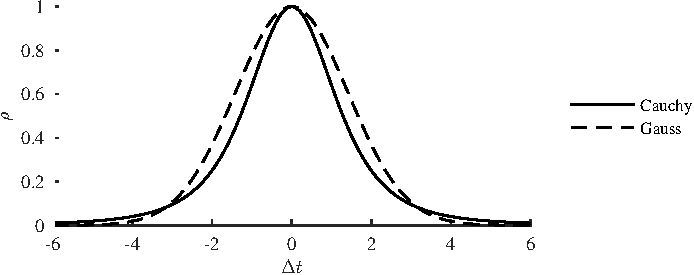
\includegraphics[]{autocorr_fun_illustration.pdf}
	\caption{Illustration of the considered autocorrelation functions.}
	\label{fig:acorr_fun}
\end{figure}

To allow direct comparison with published results and to utilize the more general Kendall's tau measure, the functions given in Eq.\ref{eq:autocorr_gauss} and \ref{eq:autocorr_cauchy} are kept and the following transformation is used:
\begin{equation}
\label{eq:tau_rho}
	\tau (\Delta t) = \frac{2}{\pi } \cdot \mathrm{asin}\left( {\rho (\Delta t)} \right).
\end{equation}
The equivalence of copulas is then set in terms of Kendall's tau values. Formula~\ref{eq:tau_rho} transforms between Pearson's rho ($\rho$) and Kendal's tau ($\tau$) for Gaussian and $t$ copulas, thus the connection to literature is established while allowing for easy extension to other copulas.

%****************************************************************************************
\subsection{Copula based dependence structure}
\label{sec:copula}

Copula is a multivariate probability distribution function with uniformly distributed marginals. It can be used to model the dependence between random variables with arbitrary marginal distributions \citep{Joe2014}. In this chapter, we deal mostly with bivariate distributions -- the formulas are given for that case -- though their extension to higher dimensions is straightforward. The copula function is expressed as:
\begin{equation}
\label{eq:copula_cdf}
	C\left( {{u_1},{u_2};\theta } \right) = {P}\left\{ {{U_1} \le {u_1},{U_2} \le {u_2}} \right\}
\end{equation}
where:

\begin{tabular}{ll}
	$C(.)$ & copula function; \\
	$\theta$ & copula parameter; \\
	$U_1, U_2$ & uniformly distributed random variables.
\end{tabular} \medskip  

\noindent
The copula function uniquely describes the dependence structure and it is independent of the marginals if those are continuous. Sklar's theorem establishes the connection between marginals, copula, and joint distribution \citep{Nelson2006, Marshall1996}:
\begin{equation}
\label{eq:sklar}
	{F_{X1X2}} = C\left( {{F_{X1}},{F_{X2}};\theta } \right)
\end{equation}
where:

\begin{tabular}{ll}
	$F_{X1}, F_{X2}$ & cumulative distribution functions of the marginals; \\
	$F_{X1X2}$ & the bivariate joint distribution.
\end{tabular} \medskip

\noindent
Copulas describe only the dependence structure of random variables, this separation of marginal and dependence is beneficial since in practice one has rarely full information about the joint distribution function, and it makes possible to separately infer the marginals and the copula.

In this chapter, Gauss, $t$, rotated Clayton, Gumbel, and rotated Gumbel copulas are adopted, all has a single parameter \citep{Nelson2006, Joe1997}. The copula functions with the range of the parameters are summarized in Table~\ref{tab:copula}. Furthermore, they are compared in Figure~\ref{fig:copula_cont}.

\begin{figure}[htbp!] 
	\centering    
	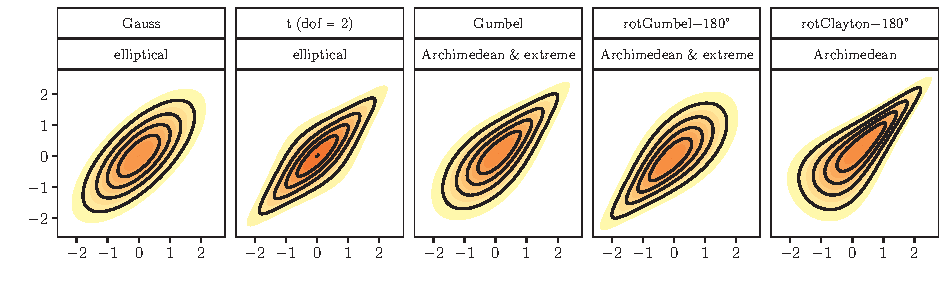
\includegraphics[]{5_copulas.pdf}
	\caption{Illustration of considered copula functions using bivariate density function contours. For all functions standard normal marginal distributions are used with 0.5 Kendall' tau.}
	\label{fig:copula_cont}
\end{figure}

The copula selection is partially motivated by their widespread use. Additionally, it is anticipated that these types cover broad range of possible functions, thus provide a representative picture about the impact of copulas on reliability. Theoretical upper and lower bounds exist for the copula functions, these are referred to as Fréchet-Hoeffding bounds \citep{Nelson2006} and they are also given in Table~\ref{tab:copula}.

Gauss (normal) and $t$ copulas belong to the elliptical family. Copulas within this family have density contours as concentric, constant eccentricity ellipses. Gumbel and Clayton copulas and their rotated alternatives belong to the Archimedean family. These are widely used due to their simple formulation and their great variety \citep{Nelson2006}. The Gumbel copula also belongs to the extreme copula family, which arises from extreme value theory, thus it can be used to model dependence between rare events \citep{Joe1997}. With the exception of Gauss copula, all considered copulas has tail-dependence, which roughly means that joint extremes are more likely than joint moderate values. Gumbel and rotated Clayton copulas have right-tale dependence, while rotated Gumbel copula has left-tail dependence. Both tails of $t$ copula exhibit tail dependence. These are also observable on the density contour plots in Figure~\ref{fig:copula_cont}, and might be of particular importance in structural reliability, which is governed by extremely rare events.

%\begin{landscape}
\begin{sidewaystable}[htbp!]
\caption{List of the considered copula functions, parameter ranges, and parameters as function of Kendall's tau ($\tau$).}
\centering
\label{tab:copula}
\small
	\begin{threeparttable}
    \begin{tabular}{llll}
    \toprule
    Name  & Copula function, $C(u_1,u_2;\theta)$ & Range of $\theta$ & $\theta(\tau)$ \\
    \midrule
    \rowcolor{lightgrey} Gauss  & ${\Phi _2}\left( {{\Phi ^{ - 1}}({u_1}),{\Phi ^{ - 1}}({u_2});\theta } \right)$ & [-1,1] & $\sin \left( {{\pi  \mathord{\left/
     {\vphantom {\pi  {2 \cdot }}} \right.
     \kern-\nulldelimiterspace} {2 \cdot }}\tau } \right)$  \\
     
     $t$  & ${t_2}\left( {{t^{ - 1}}({u_1};\nu ),{t^{ - 1}}({u_2};\nu );\theta } \right)$ & [-1,1] & $\sin \left( {{\pi  \mathord{\left/
          {\vphantom {\pi  {2 \cdot }}} \right.
          \kern-\nulldelimiterspace} {2 \cdot }}\tau } \right)$  \\
           
     \rowcolor{lightgrey} Gumbel  & $\exp \left( { - {{\left( { - \log {{({u_1})}^\theta } +  - \log {{({u_1})}^\theta }} \right)}^{{1 \mathord{\left/
       {\vphantom {1 \theta }} \right.
       \kern-\nulldelimiterspace} \theta }}}} \right)$ & [1,$\infty$] & ${1 \mathord{\left/
        {\vphantom {1 {\left( {1 - \tau } \right)}}} \right.
        \kern-\nulldelimiterspace} {\left( {1 - \tau } \right)}}$  \\ 
           
     rotGumbel-180°  & ${u_1} + {u_2} - 1 + \exp \left( { - {{\left( { - \log {{(1 - {u_1})}^\theta } +  - \log {{(1 - {u_2})}^\theta }} \right)}^{{1 \mathord{\left/
      {\vphantom {1 \theta }} \right.
      \kern-\nulldelimiterspace} \theta }}}} \right)$ & [1,$\infty$] & ${1 \mathord{\left/
              {\vphantom {1 {\left( {1 - \tau } \right)}}} \right.
              \kern-\nulldelimiterspace} {\left( {1 - \tau } \right)}}$  \\
    
     \rowcolor{lightgrey} rotClayton-180°  & ${u_1} + {u_2} - 1 + {\left( {\max \left\{ {{{\left( {1 - {u_1}} \right)}^{ - \theta }} + {{\left( {1 - {u_2}} \right)}^{ - \theta }} - 1;0} \right\}} \right)^{{{ - 1} \mathord{\left/
      {\vphantom {{ - 1} \theta }} \right.
      \kern-\nulldelimiterspace} \theta }}}$ & [-1,$\infty$]$\setminus \left\{ 0 \right\}$ & ${{2 \cdot \tau } \mathord{\left/
       {\vphantom {{2 \cdot \tau } {\left( {1 - \tau } \right)}}} \right.
       \kern-\nulldelimiterspace} {\left( {1 - \tau } \right)}}$  \\           
     
    lower bound, $C_\mathrm{sup}$  & $\max \left\{ {1 - 2 + {u_1} + {u_2};0} \right\}$ & -- & --  \\
    
    \rowcolor{lightgrey} upper bound, $C_\mathrm{inf}$  & $\min \left\{ {{u_1};{u_2}} \right\}$ & -- & --  \\
              
    \bottomrule
    \end{tabular}
    \begin{tablenotes}
    	\item $\Phi_2(.)$ and $\Phi(.)$  are the bi- and univariate standard normal cumulative distribution functions.
    	\item $t_2(.)$ and $t(.)$ are the bi- and univariate $t$ cumulative distribution functions with $\nu = 2$ degrees of freedom.
    	\item -- Not applicable/not available. 
   	\end{tablenotes}
   	\end{threeparttable}
\end{sidewaystable}
%\end{landscape}



%****************************************************************************************
%****************************************************************************************
\section{PHI2 method}

PHI2 method is an algorithm to solve time-variant reliability problems where (\textit{i}) a random variable is monotonically changing in time, e.g. degradation of material properties; and/or (\textit{ii}) a continuous time-varying process is involved. The algorithm originates from \citet{Hagen1991}, who formulated the calculation of the out-crossing rate as a two-component, parallel system reliability problem (Eq.\ref{eq:out_cross}).
Out-crossing occurs if a random variable or stochastic process is passing the limit state function from safe- to failure region. By definition, the out-crossing rate in time is given as \citep{Hagen1991}:
\begin{equation}
\label{eq:out_cross}
	{\nu ^ + }(t) = \mathop {\lim }\limits_{\Delta t \to 0} \frac{{P\left( {\left\{ {g(t) > 0} \right\}\bigcap {\left\{ {g(t + \Delta t) \le 0} \right\}} } \right)}}{{\Delta t}}
\end{equation}
where:

\begin{tabular}{ll}
	$\nu ^+$ & out-crossing rate; \\
	$g(.)$ & limit state function; \\
	$t$ & monotonically increasing parameter, typically time.
\end{tabular} \medskip

\noindent
Since in structural engineering out-crossings occur rarely, it is generally assumed that they can be described with a Poisson process \citep{Cramer1967}. After some algebra and simplification one can derive the formula that is widely used in structural reliability to calculate time-variant failure probability \citep{Melchers2002}:
\begin{equation}
\label{eq:P_f_t}
	{P_{\mathrm{f}}}(t) = {P_{\mathrm{f}}}(0) + \int\limits_0^t {{\nu ^ + }(\tau )}  \cdot {\mathrm{d}}\tau.
\end{equation}
The nominator in Eq.\ref{eq:out_cross} expresses the failure probability of a parallel system with correlated components. This system reliability problem inherits the copula assumption of the stochastic process. The correlation is typically estimated from the sensitivity factors obtained by first order reliability analysis (FORM) and then bivariate normal distribution is used to calculate the system failure probability \citep{Renaud2004}. Likely this is why the method is coined as PHI2 by \citet{Renaud2002}. However, the method is more general and not restricted to bivariate normal distribution, thus the naming is not fortunate. Nevertheless, it reflects well the overwhelming use of Gauss copulas in structural reliability. The application of Gauss copula in classical reliability methods such as FORM is usually referred to as Nataf transformation \citep{Liu1986, Nataf1962}.

It is known that the out-crossing rate given by Eq.\ref{eq:out_cross} is sensitive to the size of the time step ($\Delta t$), thus \citet{Sudret2008anal} derived an improved formula, which considerably mitigates this. Since it also relies on the Gauss copula assumption, the original, numerical derivation (Eq.\ref{eq:out_cross}) version is adopted here. To minimize the error, Sudret recommends the time step to be taken as 10\% of the correlation length ($\tau_\mathrm{F}$). Our analysis confirms this recommendation for Gauss copula with double precision calculation. However, for other copulas the results can be greatly sensitive to the chosen time step. To alleviate this problem multiprecision calculation -- quad or larger \citep{mct2016}  -- is adopted that yields to numerically stable results even for small time steps. For the examples in this chapter the range $\Delta t = \left( {{{10}^{ - 5}} \div {{10}^{ - 3}}} \right) \cdot {\tau _F}$  is found to have stable convergence: (\textit{i}) the time step is sufficiently small to accurately estimate the derivative (Eq.\ref{eq:out_cross}); and (\textit{ii}) the floating point representation is accurate enough to keep truncating errors low. Thus, for all calculations time step in this range is applied, the convergence and sensitivity to discretization are checked in each cases.

The system reliability problems emerging in PHI2 method are formulated with different copulas and solved by direct, numerical integration (DI). This approach is suited only for simple problems, such those considered in this chapter. For more complicated problems computationally more efficient methods would be needed such as FORM or SORM. Note, that these methods are almost solely implemented with Nataf transformation (Gauss copula) in the currently available research and commercial applications. They can be extended to elliptical copulas, since for these the physical variables can be transformed to a space where the search for the most probable point reduces to minimal distance search \citep{Lebrun2009}. However, to date, for other copula types no generalization of these methods is available, thus the application of non-elliptical copulas might be unmanageable.

%****************************************************************************************
%****************************************************************************************
\section{Example 1: simple time-variant problem}

First, a simple example is analyzed with a single continuous stochastic process ($S(t)$) and deterministic resistance ($R$). The limit state function is linear and expressed by Eq.\ref{eq:gfun_ex1}:
\begin{equation}
\label{eq:gfun_ex1}
	g(t) = R - S(t). 
\end{equation}
Using Eq.\ref{eq:out_cross}, the system failure probability ($P_\mathrm{f,sys}$), required in PHI2 method can be written as:
\begin{equation}
\label{eq:P_f_sys}
	{P_{{\mathrm{f,sys}}}} = {{P}}\left( {\left\{ {R - {S_1} > 0} \right\}\bigcap {\left\{ {R - {S_2} \le 0} \right\}} } \right).
\end{equation}
Where $S_1$ and $S_2$ are correlated random variables defined as:
\begin{equation}
\label{eq:S_def}
	{S_1} = S(t) \text{\quad and \quad} {S_2} = S(t + \Delta t). 
\end{equation}
Using Eq.\ref{eq:P_f_sys} and \ref{eq:sklar}, the failure probability of the parallel system can be expressed as:
\begin{equation}
\label{eq:P_f_sys_ex1}
	\begin{aligned}
		{P_{{\mathrm{f,sys}}}} &= {F_S}\left( R \right) - {F_{S1S2}}\left( {R,R} \right)\\
		 & = {P_{{\mathrm{s,comp}}}} - C\left( {{P_{{\mathrm{s,comp}}}},{P_{{\mathrm{s,comp}}}};\theta } \right)
	\end{aligned}
\end{equation}
where $P_\mathrm{s,comp}$ stands for the survival probability of a component and it corresponds to $1-P_\mathrm{f}(0)$. It can be seen from Eq.\ref{eq:P_f_sys_ex1} that for a given $P_\mathrm{s,comp}$ the system's failure probability is independent of the marginal distributions. Therefore, the stochastic process is sufficiently characterized by the autocorrelation function and by the copula, for the current purposes.

By specifying $P_\mathrm{s,comp}$ and the copula type, the system's failure probability can be calculated. Then by the finite difference formulation of Eq.\ref{eq:out_cross} and using Eq.\ref{eq:P_f_t} the time-variant reliability can be obtained. For this example, the time interval is taken as 50 years, and the autocorrelation length is $\tau_\mathrm{F} = 1/365$ year. First, Gaussian autocorrelation function is used.

The analyses are completed for various initial/component failure probabilities ranging from $10^{-10}$ to $10^{-6}$ with all five copulas having the same Kendall's tau for a particular set of input parameters. The results are represented as reliability indices in Figure~\ref{fig:beta_ex1}. Moreover, Figure~\ref{fig:pf_ex1} summarizes the time-variant failure probabilities and their normalized values.

\begin{figure}[htbp!] 
	\centering    
	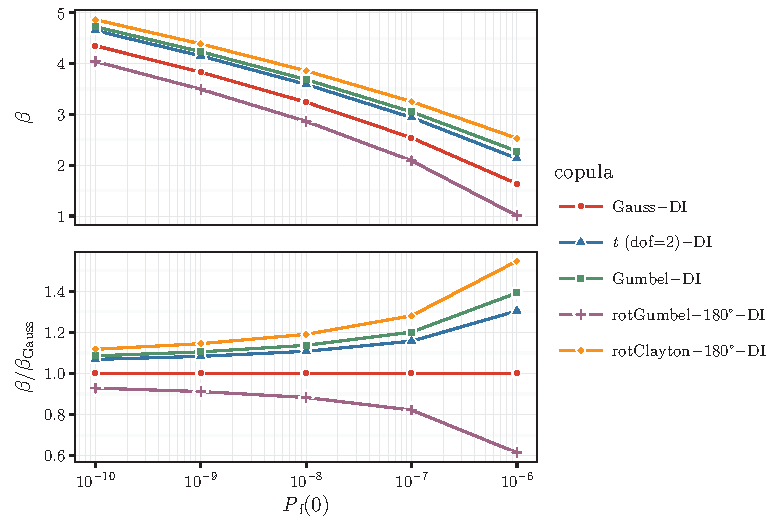
\includegraphics[]{simple_example_beta.pdf}
	\caption{Reliability indices ($\beta$) and normalized reliability indices plotted against initial failure probability ($P_\mathrm{f}(0)$) for various copulas. DI refers to direct integration.}
	\label{fig:beta_ex1}
\end{figure}

\begin{figure}[htbp!] 
	\centering    
	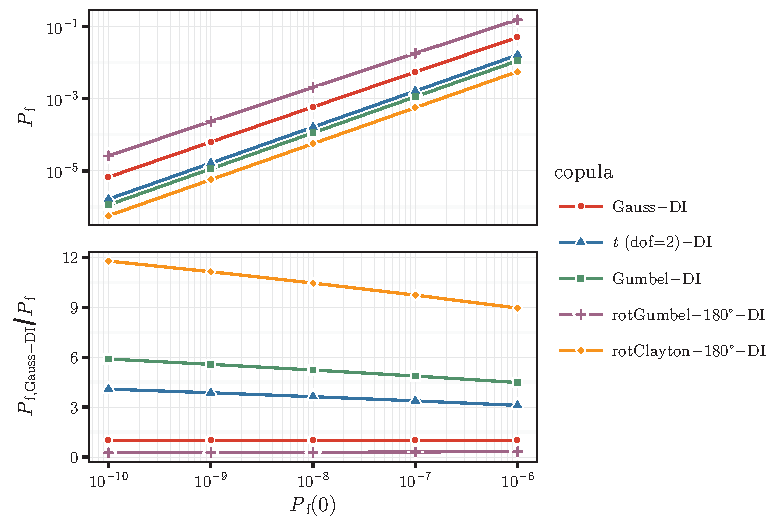
\includegraphics[]{simple_example_Pf.pdf}
	\caption{Failure probabilities ($P_\mathrm{f}$) and normalized failure probabilities plotted against initial failure probability ($P_\mathrm{f}(0)$) for various copulas. DI refers to direct integration.}
	\label{fig:pf_ex1}
\end{figure}

From the figures it is clear that the copula type has significant effect on the failure probability. Compared with the widely used Gauss, the rotated Gumbel copula gives 3.1-3.9 times higher failure probability, the ratio is decreasing with decreasing initial failure probability. On the other hand, $t$, Gumbel, and rotated Clayton copulas yield to 0.09-0.33 times lower results than the Gauss copula; here too the ratio is decreasing with decreasing initial failure probability. Irrespectively of the copula type, the initial failure probability has no significant effect on the normalized results.

The calculations are repeated with other correlation lengths ranging from 0.1/365 to 100/365. It is found that the normalized results are only slightly affected by this change, even at maximum less than 2\% change is observed in failure probability. This can be explained by that (\textit{i}) the correlation between $S_1$ and $S_2$ is independent of $\tau_\mathrm{F}$ because $\Delta t$ is chosen as a fixed percentage of that; and (\textit{ii}) $P_\mathrm{f}(0)$ is typically much smaller than the second term in Eq.\ref{eq:P_f_t}. Indeed, the largest difference is observed when $P_\mathrm{f}(0)$ is comparable to the time-variant failure probability. In case of $\tau _\mathrm{F} = 1000/365$ for Gumbel copula, the normalized time-variant failure probability increases by 7\% compared to 1/365 year correlation length. The increase is 15\% for rotated Clayton copula.

Up to this point, all presented calculations correspond to Gaussian autocorrelation function. Switching to Cauchy function, the normalized time-variant failure probabilities -- with $\tau_\mathrm{F} = 1/365$ year correlation length -- change irrespectively of initial failure probability and of copula type. The ratio of normalized time-variant Cauchy and Gaussian failure probabilities is uniformly 1.41. It is solely influenced by the autocorrelation function.

In our case, the upper Fréchet-Hoeffding bound yields to zero up-crossing rate, while the lower bound gives infinitely large value. These can be shown using Eq.\ref{eq:P_f_sys_ex1} and Table~\ref{tab:copula}:
\begin{equation}
	\begin{split}
		\begin{aligned}
			{P_{{\mathrm{f,sys,inf}}}} &= {P_{{\mathrm{s,comp}}}} - {C_{\sup }}\left( {{P_{{\mathrm{s,comp}}}},{P_{{\mathrm{s,comp}}}}} \right) = 3 \cdot {P_{{\mathrm{s,comp}}}} - 1\\
			{P_{{\mathrm{f,sys,sup}}}} &= {P_{{\mathrm{s,comp}}}} - {C_{\inf }}\left( {{P_{{\mathrm{s,comp}}}},{P_{{\mathrm{s,comp}}}}} \right) = 0
		\end{aligned}
	\end{split}
		\begin{split}
			\begin{aligned}
				\xrightarrow[]{{\frac{{{\mathrm{d}}{P_{{\mathrm{f,sys}}}}(t)}}{{{\mathrm{d}}\Delta t}}}} \nu _{\inf }^ +  &= \infty \\
				\xrightarrow[]{{\frac{{{\mathrm{d}}{P_{{\mathrm{f,sys}}}}(t)}}{{{\mathrm{d}}\Delta t}}}} \nu _{\sup }^ +  &= 0.
			\end{aligned}
		\end{split}
\end{equation}
This means that the copula bounds convey no useful information; however, more importantly it implies that there are copula functions that yields to arbitrary large or arbitrary small out-crossing rates. Hence, compared with Gauss copula, arbitrary large error could be produced.

%****************************************************************************************
%****************************************************************************************
\section{Example 2: corroding beam}

The following example is adopted from \citet{Sudret2008anal}. It is a simply supported, corroding steel beam subjected to a time-variant load that is described by a continuous stochastic process (Figure~\ref{fig:corr_beam}). The original example is intended to illustrate the application of PHI2 method to solve a time-variant reliability problem and it implicitly adopted Gauss copula. Herein we extend the example by investigating the effect of copula function on out-crossing rate and reliability.

\begin{figure}[htbp!] 
	\centering    
	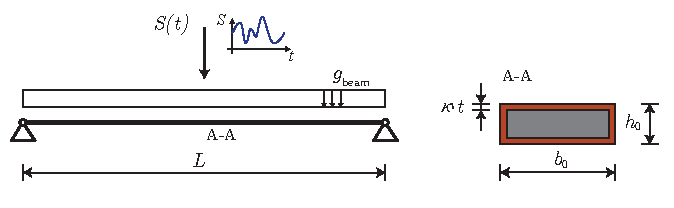
\includegraphics[]{corroding_beam_illustration_.pdf}
	\caption{Illustration of the corroding beam example.}
	\label{fig:corr_beam}
\end{figure}

The mechanical and probabilistic models (Table~\ref{tab:prob_models_corr_beam}) are the same as in the original example, solely the copula is varied that describes the dependence between the survival and failure of the structure between two ``close'' time instants.

\begin{table}[htbp!]
\caption{Probabilistic models for corroding beam example.}
\centering
\label{tab:prob_models_corr_beam}
\small
	\begin{threeparttable}
    \begin{tabular}{llll}
    \toprule
    Variable name  & Distribution & Mean & CV\\
    \midrule
    \rowcolor{lightgrey} Concentrated load, $S(t)$ [N]  & Normal & 3500 & 0.20  \\
    Yield strength, $\sigma_\mathrm{R}$ [MPa]  & Lognormal & 240 & 0.10  \\
    \rowcolor{lightgrey} Beam width, $b_0$ [mm]  & Lognormal & 200 & 0.05  \\
    Beam height, $h_0$ [mm]  & Lognormal & 40 & 0.10  \\
    \rowcolor{lightgrey} Unit weight, $\rho_\mathrm{st}$ [kN/$\mathrm{m}^3$]  & constant & 78.5 & --  \\
    Span, $L$ [m]  & constant & 5 & -- \\
    \bottomrule
    \end{tabular}
    \begin{tablenotes}
    	\item -- Not applicable.
    \end{tablenotes}
    \end{threeparttable}
\end{table}

The autocorrelation function of the stochastic process is Gaussian (Eq.\ref{eq:autocorr_gauss}), with correlation length of 1 day. The corrosion occurs uniformly on the surface of the beam and propagates linearly in time:
\begin{equation}
	b(t) = {b_0} - 2 \cdot \kappa  \cdot t \text{\quad and \quad} h(t) = {h_0} - 2 \cdot \kappa  \cdot t 
\end{equation}
where:

\begin{tabular}{ll}
	$t$ & time; \\
	$\kappa$ & corrosion rate, 0.05 mm/year.
\end{tabular} \medskip

\noindent
Taking into account the self-weight of the beam and the time-variant load ($S(t)$) the limit state function corresponding to the formulation of a plastic hinge at midspan is given by Eq.\ref{eq:gfun_corr_beam}:
\begin{equation}
\label{eq:gfun_corr_beam}
	\begin{aligned}
		g(t) &= {M_{\mathrm{R}}}(t) - \left( {{M_{\mathrm{G}}} + {M_S}(t)} \right)\\
		& = \frac{{b(t) \cdot h{{(t)}^2} \cdot {\sigma _{\mathrm{R}}}}}{4} - \left( {\frac{{{\rho _{{\mathrm{st}}}} \cdot {b_0} \cdot {h_0} \cdot {L^2}}}{8} + \frac{{S(t) \cdot L}}{4}} \right).
	\end{aligned}
\end{equation}
In accordance with the original example, the self-weight is assumed to be time-invariant, although the cross-section's dimensions are decreasing in time. The design life of the beam is assumed to be 20 years.

The time-variant reliability problem is solved with copulas listed in Table~\ref{tab:copula}; the corresponding out-crossing rates and normalized out-crossing rates in time are shown in Figure~\ref{fig:outcross_ex2}. In case of Gauss copula, besides the direct numerical integration (DI) the calculations are also carried out by FORM. In the latter, the correlation between the two components (Eq.\ref{eq:out_cross}) is estimated from the angle between corresponding FORM hyperplanes \citep{Ditlevsen1979bounds}. The small difference between FORM and numerical integration outcomes is attributed (\textit{i}) to the non-linearity of limit state function; and (\textit{ii}) to the approximate correlation coefficient used in FORM. The results confirm the applicability of FORM to approximate the reliability.

\begin{figure}[htbp!] 
	\centering    
	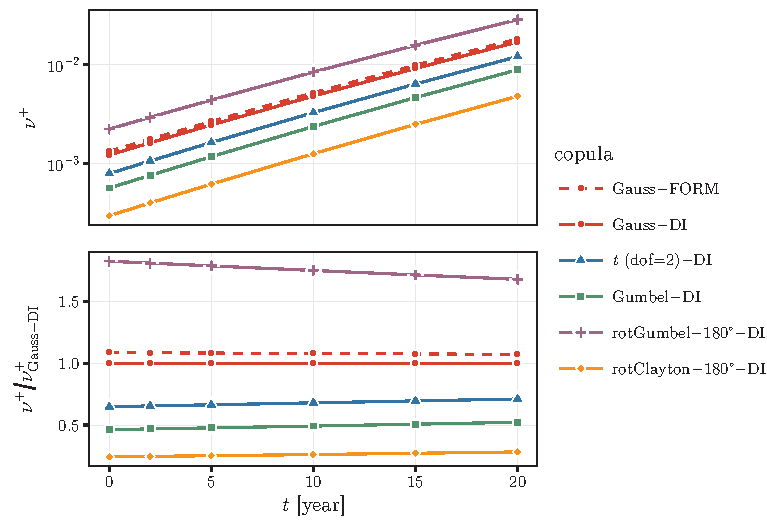
\includegraphics[]{Sudrets_beam_log_nu.pdf}
	\caption{Out-crossing rates ($\nu ^+$) and normalized out-crossing rates in time for various copulas. DI refers to direct integration.}
	\label{fig:outcross_ex2}
\end{figure}

Figure~\ref{fig:outcross_ex2} shows considerable differences in out-crossing rates for different copulas. Compared with the Gauss-DI solution, the rotated Gumbel copula gives about 1.8 times larger rates, while other copulas lead to smaller rates. The largest reduction is observed for rotated Clayton copula, which is 0.25 times that of the Gauss copula. It can be also observed that normalized out-crossing rates vary only slightly in time.

Figure~\ref{fig:Pf_ex2} and Figure~\ref{fig:beta_ex2} illustrate the time-variant failure probabilities and reliability indices, respectively. The former follows well the trend observed in out-crossing rates, which is as quasi-constant ratio in time. In Figure~\ref{fig:Pf_ex2}, it can be seen that the normalized ratios per copula function is very close to that of the out-crossing rates, with the exception of $t=0$ time instant, where the out-crossing rate is not taken into account. The figures also indicate that the two degrees of freedom $t$ copula leads to similar results as of Gumbel copula. Compared with the Gauss copula with direct integration, the largest ratios in failure probabilities are 1.1 and 1.8 for Gauss-FORM and rotated Gumbel copulas, respectively. The smallest ratios are 0.7, 0.5, and 0.3 for $t$, Gumbel, and rotated Clayton copulas, respectively. The increasing difference in reliability indices with increasing time is attributed to the nonlinear transformation between failure probability and reliability index.

\begin{figure}[htbp!] 
	\centering    
	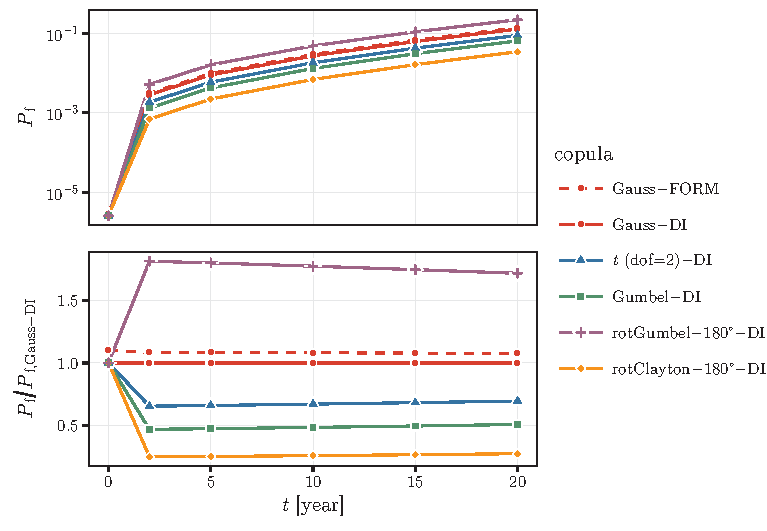
\includegraphics[]{Sudrets_beam_log_Pf.pdf}
	\caption{Failure probabilities ($P_\mathrm{f}$) and normalized failure probabilities in time for various copulas. DI refers to direct integration.}
	\label{fig:Pf_ex2}
\end{figure}

\begin{figure}[htbp!] 
	\centering    
	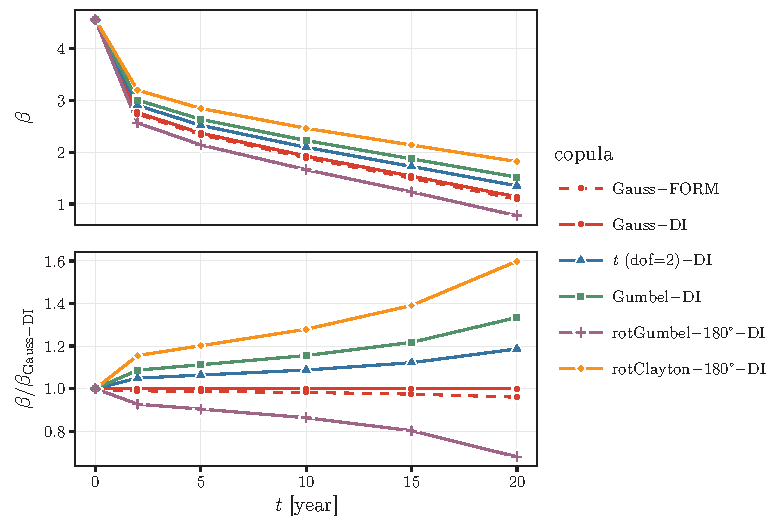
\includegraphics[]{Sudrets_beam_beta.pdf}
	\caption{Reliability indices ($\beta$) and normalized reliability indices for various copulas. DI is referring to direct integration.}
	\label{fig:beta_ex2}
\end{figure}

All the presented results are from analyses using Gaussian autocorrelation function. The calculations are repeated with Cauchy autocorrelation function and the outcomes show that the change in out-crossing rate is independent of the copula type and time. The ratio of out-crossing rate obtained by using Cauchy and Gaussian autocorrelation functions is 1.41. This considerable effect is also rarely acknowledged in the literature, where the Gaussian autocorrelation function is prevalent. This ratio is inherited by the time-variant failure probability since the initial failure probability is negligible compared to the term involving the out-crossing rate (Eq.\ref{eq:P_f_t}).

%****************************************************************************************
%****************************************************************************************
\section{Example 3: generic structure subject to snow load}
\label{sec:copula_snow}

In this example a time-variant reliability problem is studied, where the stochastic process is inferred from observations. Maximum likelihood method (Section~\ref{subsec:point estiamtes}) is chosen for parameter estimation. However, the calculation of the full likelihood is computationally demanding -- often numerically intractable -- even for moderately large datasets due to the need to evaluate high-dimensional, multivariate distributions. Thus, it is often replaced with pairwise likelihood that requires only bivariate distributions and shares the same properties as the full likelihood based estimator except its loss of efficiency \citep{PadoanRibatetSisson2010}. This pairwise approach is also applied for spatial modeling such as temperature extremes in Switzerland \citep{Ribatet2012} and adopted herein too. The formulation of the pairwise likelihood function is given as:
\begin{equation}
	{L_{\mathrm{p}}}\left( {{\bf{x}};{\bf{\theta }}} \right) = \prod\limits_{i < j} {p\left( {\left[ {{x_i},{x_j}} \right];{\bf{\theta }}} \right)}.
\end{equation}
Ground snow observations in the form of snow water equivalent are selected for the representative lowland location of Budapest in the Carpathian Region. The data are from the CarpatClim database and available in 10~km spatial and 1-day maxima temporal resolution \citep{Szalai2013}. Budapest (19.1°E, 47.5°N) is characterized by intermittent snow cover, i.e. couple of snowfalls followed by often complete melting. The analyzed sample is extracted using the following principles:
\begin{itemize}
	\item peaks are extracted from daily maxima;
	\item from two peaks separated by four or less days the smaller one is removed;
	\item each winter season is treated as a single unit because snowfalls are clustered over a few months;
	\item if only a single peak occurs in a season its likelihood is calculated from the univariate marginal.
\end{itemize}
This means that a sequence of peaks is obtained for each winter seasons that are assumed to be independent. However, peaks within the same season are treated as realizations of a time-continuous stochastic process, thus they are dependent. The extracted sequence of peaks along with daily maxima are illustrated in Figure~\ref{fig:peak_sample_ex3} for five consecutive years.

\begin{figure}[htbp!] 
	\centering    
	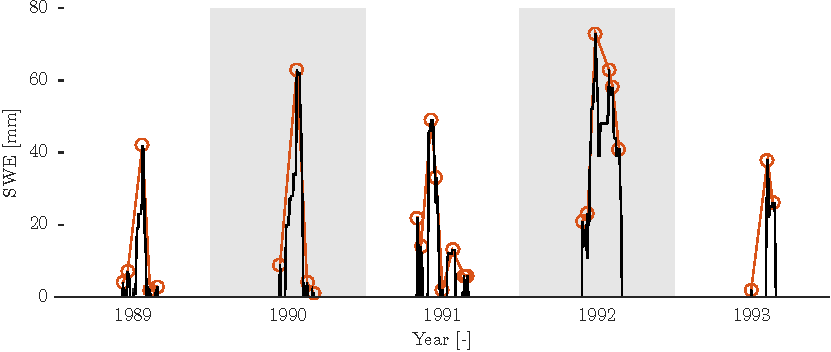
\includegraphics[]{sample_&_peaks.pdf}
	\caption{Illustration of extracted peaks from daily snow water equivalent (SWE) maxima over five consecutive years.}
	\label{fig:peak_sample_ex3}
\end{figure}

Note that this is a somewhat arbitrary approach and the sample could be extracted many different ways. However, this deemed sufficient to illustrate the effect of copulas inferred from data. In average five peaks are present for a given winter season and in total there are 249 peaks for the 49 seasons. Gauss and Cauchy autocorrelation functions, and Gauss, $t$, Gumbel, rotated Gumbel, and rotated Clayton copulas are considered. Additionally, three marginal distributions are used: Gauss, Lognormal, and Gumbel.

For each autocorrelation-marginal-copula triplet three parameters are inferred: two parameters of the marginal and the correlation length. Separate inference of the marginal and copula is not possible due to nature of the problem, thus the parameters are estimated simultaneously.

Akaike information criterion (AIC, Eq.\ref{eq:AIC}) is calculated for each triplet. Then pooling is made for each autocorrelation-marginal sets, where a set is composed of the copulas as candidate models. This pooling is explained by the large difference in AIC (>100) between models with different marginal function. The related Akaike weights ($w$, Eq.\ref{eq:Akaike_weight}) are visually compared in Figure~\ref{fig:akaike_ex3}. It shows that -- with the exception of Gauss autocorrelation-Gumbel marginal pair -- Gumbel copula performs significantly better than the other considered copulas.

\begin{figure}[htbp!] 
	\centering    
	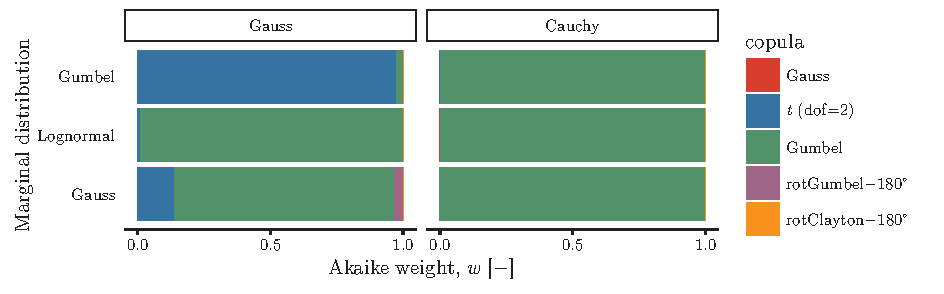
\includegraphics[]{akaike_weights.pdf}
	\caption{Akaike weights for autocorrelation-marginal pools. A pool is formed by a particular autocorrelation function (Gauss, Cauchy) and by a particular marginal distribution (Gauss, Lognormal, Gumbel), and the six copula functions provide the candidate models.}
	\label{fig:akaike_ex3}
\end{figure}

In most cases, the Cauchy autocorrelation function provides significantly better fit ($\Delta \mathrm{AIC} > 5$) than the Gauss using the same type of copula and type of marginal. The only exception is the rotated Clayton copula for which Gauss autocorrelation function is slightly better. The marginal distribution type has substantial effect on the fit, it can yield to over 100 difference in AIC. Lognormal provides the best fit, followed by Gumbel and Gauss.
The outstanding performance of Gumbel copula implies that extreme copulas might suit better for describing dependent extremes, this conjecture is also supported by the extreme value theory. Furthermore, by using extreme $t$ copula with two degrees of freedom even better fit is obtained than that of Gumbel.

To explore the effect on time-variant reliability the inferred stochastic models are used in a simple reliability problem characterized by the following limit state function:
\begin{equation}
	g(t) = R - \left( {G + S(t)} \right).
\end{equation}
The properties of the involved probabilistic models are summarized in Table~\ref{tab:prob_models_snow_stoch}.

\begin{table}[htbp!]
\caption{Marginal distribution of random variables for stochastic snow load example.}
\centering
\label{tab:prob_models_snow_stoch}
\small
	\begin{threeparttable}
    \begin{tabular}{llll}
    \toprule
    Variable name  & Distribution & Mean & CV \\
    \midrule
    \rowcolor{lightgrey} Resistance, $R$  & Lognormal & 250 & 0.10  \\
    Permanent action, $G$  & Normal & 60 & 0.07  \\
    \rowcolor{lightgrey} Snow maxima, $S(t)$  & Normal, Lognormal, Gumbel & \tnote{*} & \tnote{*}  \\
    \bottomrule
    \end{tabular}
    \begin{tablenotes}
    	\item[*] Depends on the applied autocorrelation-marginal-copula triplet.  
   	\end{tablenotes}
   	\end{threeparttable}
\end{table}

For comparison, the out-crossing rates are calculated for each triplet and presented in a normalized form in Figure~\ref{fig:norm_nu_ex3}. For each marginals the out-crossing rates are normalized with that of the corresponding Gauss copula. The same trend is observed for all marginals. Using Gauss copula the largest underestimation of out-crossing rate is 8 times, while the largest overestimation is 3 times. Neither of these are corresponding to Gumbel copula, which yields to 4.2, 2.9, and 3.5 times smaller out-crossing rates for Gauss, Lognormal, and Gumbel marginals, respectively. Figure~\ref{fig:norm_nu_ex3} conceals the multiple order of difference between out-crossing rates of different marginals. Although it is low importance now as we are interested in the effect of copula functions. The effect of replacing the Gauss autocorrelation with Cauchy function yields to similar results as observed in previous examples. The ratio of corresponding Cauchy and Gauss out-crossing rates is uniformly about 1.4.

\begin{figure}[htbp!] 
	\centering    
	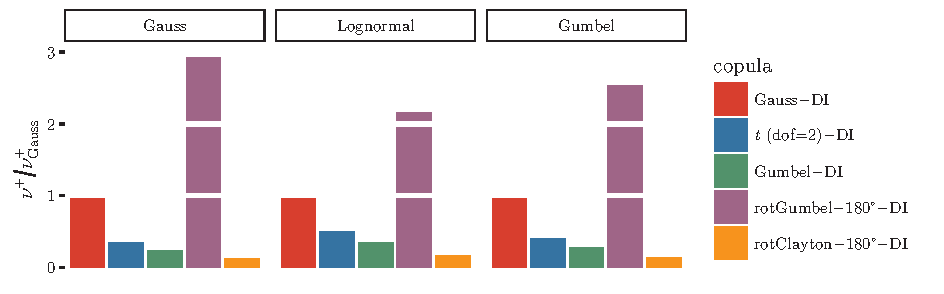
\includegraphics[]{normalized_nu_p.pdf}
	\caption{Normalized out-crossing rates for Gauss autocorrelation function. For each marginals (Gauss, Lognormal, Gumbel) the out-crossing rates are normalized with that of the corresponding Gauss copula. DI refers to direct integration.}
	\label{fig:norm_nu_ex3}
\end{figure}

\section{Application example: Eiffel-hall of Budapest}
In Section~\ref{sec:copula_snow} a generic structure is analyzed, which is located at the site of Eiffel-hall. Herein the same location -- thus same snow action -- but the structure of the Eiffel-hall is investigated. The structure is introduced in Annex~\ref{sec:eiffel}, here only the essential details, which are required to interpret the results, are provided. The stochastic snow models fitted in the preceding section is used in the analysis. Only Gaussian autocorrelation function and Gumbel marginal distribution are considered. The wind action is represented by a distribution function corresponding to 50 years reference period. The out-crossing rates -- calculated by direct numerical integration -- are summarized in Table~\ref{tab:eiffel_nu_p}. Compared with Gauss copula, the largest difference is observed for Gumbel copula, which yields to about three times smaller out-crossing rate. Figure~\ref{fig:akaike_ex3} shows that for the inputs the $t$ copula provides the best fit, which leads to 40\% smaller out-crossing rate than that of the Gauss. The effect of copula function type is smaller than in previous examples, though it is still considerable.

\begin{table}[htbp!]
\caption{Out-crossing rates for Eiffel-hall considering Gauss autocorrelation function and Gumbel marginal distribution.}
\centering
\label{tab:eiffel_nu_p}
\small
    \begin{tabular}{llllll}
    \toprule
    Parameter  & Gauss & $t$ (dof=2) & Gumbel & rotGumbel-180° & rotClayton-180°\\
    \midrule
    \rowcolor{lightgrey} $\nu^+$ [$\cdot 10^{-3}$]  & 1.18 & 0.737 & 0.403 & 2.22 & 0.794  \\
    $\nu^+/\nu_\mathrm{Gauss}^+$  & 1.00 & 0.622 & 0.340 & 1.87 & 0.671 \\
    \bottomrule
    \end{tabular}
\end{table}

%****************************************************************************************
%****************************************************************************************
\section{Discussion}

Dependence structure (or copula function) uncertainty belongs to probability model selection uncertainty. Thus, from mathematical point of view the issue is very similar to distribution selection uncertainty, which is treated in Chapter~\ref{cha:stat_unc}. The same considerations apply here as well: typically there are insufficient data to identify the true model, copula function. Hence, for normal structures agreement on the copula function is recommended, and for safety critical structures Bayesian model averaging is advocated to account for copula type uncertainty.

For non-Gaussian copulas direct integration is used here and typically quad or larger  precision calculation is required to achieve convergence. Efficient algorithms, such as FORM, are currently only available for elliptical copulas, additional research would be needed to extend existing or develop new methods for other copulas. Thus, this poses a limitation on incorporation of copula function uncertainty in probabilistic analysis.

%****************************************************************************************
%****************************************************************************************
\section{Summary and conclusions}

In this chapter the effect of the dependence structure between random variables is analyzed on the failure probability of structures. Copula function is adopted to describe the dependence and the emphasis is placed on time-variant reliability using PHI2 method. The analysis of three simple examples -- considering Gauss, $t$, rotated Clayton, Gumbel, and rotated Gumbel copulas -- reveal:
\begin{itemize}
	\item The applied dependence structure has significant effect on time-variant reliability. The prevalently applied Gauss copula assumption can 4 times underestimate or even 10 times overestimate failure probabilities obtained by other adopted copulas.
	\item For a simple case (Example 1), it is demonstrated that by an appropriate choice of copula function arbitrary large error can be produced in out-crossing rate, compared with that of the Gauss copula.
	\item The correlation length of stochastic process and initial failure probability have minor effect on the ratio of the Gauss and other copula results.
	\item The autocorrelation function has considerable effect on the time-variant failure probability. The ratio of normalized time-variant Cauchy and Gaussian failure probabilities is uniformly 1.41. It is solely influenced by the autocorrelation function.
	\item Analysis of ground snow observations implies that extreme copulas, such as Gumbel, fit significantly better to dependent snow extremes than Gauss copula. The Gumbel copula can yield to 4 times lower out-crossing rate than that of Gauss.
\end{itemize}
	
To our knowledge the copula and autocorrelation effects have not yet been studied previously and the findings provide a novel insight into time-variant problems.
The results also give indication about whether a particular part of the mechanical or probabilistic model is worth of refinement, if the actual dependence structure is largely unknown.

If observations are available, the actual dependence structure should be inferred, and in case of limited information, multiple copula functions should be used to quantify the related uncertainty. Model averaging (Annex~\ref{subsec:model_averaging}) provides a viable approach to rigorously account for this uncertainty. In reporting of reliability analyses, the dependence structures, namely the adopted copulas should also be reported to give full description of the probabilistic model and to allow reproducibility.